\documentclass{article}
\usepackage{titlesec}
\usepackage{mhchem}
\usepackage{array}
\usepackage{graphicx}
\usepackage[bmargin=2cm, tmargin=2cm]{geometry}
\usepackage{fourier-orns}
\usepackage{amsfonts}
\usepackage{amssymb}
\usepackage{amsmath}
\usepackage{physics}
\usepackage{modiagram}


\newcommand{\thedate}[1]{\hfill{\small\sc #1}}
\newcommand{\NB}{{\large\lefthand}\quad}
\newcommand{\cm}{cm\(^{-1}\) }
\newcommand{\mcm}{\text{ cm}^{-1}}
\titleformat{\section}[runin]{\sc\Large}{\S\thesection}{3ex}{}[]
\titleformat{\subsection}[hang]{\sc\large}{\S\thesubsection}{3ex}{}[]
\titleformat{\subsubsection}[hang]{}{\S\thesubsubsection}{1ex}{\bfseries}[]

\newtheorem{defn}{Definition}[section]

\title{Energy, Spectroscopy and Solid State Chemistry}
\date{}
\author{}
\begin{document}
    \maketitle
    \section{Spectroscopy}
    \subsection{Introduction}\thedate{28/10/20 --- Week 1}
    \subsubsection{The Born-Oppenheimer Approximation}
    The assumption that the electronic motion and the nuclear motion in molecules can be separated, due to the
    difference in mass between the electron and the nuclei.
    \begin{align*}
        \Psi_{tot} &= \psi_{el} \psi_{nuc}\\
        \text{Where the resulting total} & \text{ energy is a simple sum.}\\
        E_{tot} &= E_{el} + E_{nuc}
    \end{align*}
    It is very convinient, although slightly less rigorous, to factorise \(\Psi_{nuc}\) into vibrational and
    rotational parts. Translational energy is unquantised and so useless for spectroscopy.
    \begin{align*}
        \Psi_{tot} &= \psi_{el} \psi_{vib} \psi_{rot}\\
        E_{tot} &= E_{el} + E_{vib} + E_{rot}
    \end{align*}
    \begin{figure}[h]
        \centering
        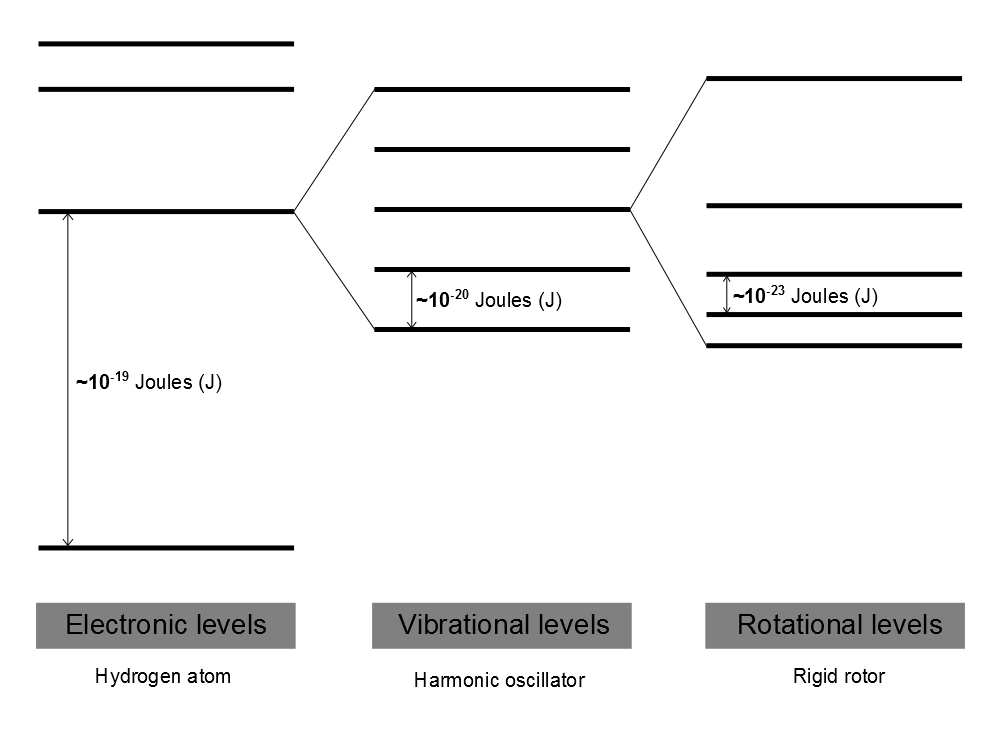
\includegraphics[width=10cm]{trans.png}
        \caption{Transitions of different energy levels}
    \end{figure}

    \begin{tabular}[2cm]{l l l l}
        \(\Delta \text{E} \approx \) \hspace{1cm}  & \(10^{4} - 10^{5} \text{cm}^{-1}\) \hspace{0.8cm} & \(10^{2} - 10^{3} \text{cm}^{-1}\) \hspace{0.8cm} & \(0.1 - 10 \text{cm}^{-1}\)\\
        Transitions at \(\Delta \lambda \approx \) & \(500 - 100 \text{nm}\) \hspace{0.5cm} & \(100 - 2 \mu \text{m} \) \hspace{0.5cm} & \(10 \text{cm} - 1 \text{mm}\)\\
        Light range & Vis-UV & Infrared & Microwave\\
    \end{tabular}

    \vspace{1cm}
    Every electronic energy level contains multiple vibrational levels which contains multiple rotational levels.
    More on this to come. 

    \subsubsection{The Boltzmann Law} At thermal equilibrium the relativep population of the \(i^{\text{th}}\) energy level is given by:
    \begin{align*}
        \frac{n_i}{n_0} = \frac{g_i}{g_0}e^{-\frac{\Delta E_i}{k_B T}}
    \end{align*}
    \begin{itemize}
        \item \(g_i\) is the degeneracy of the \(i\)th level (the number of states with the same energy)
        \item \(\Delta E_i\) is the energy difference between the lowest (ground) and \(i\)th levels
        \item \(k_B\) is the Boltzmann constant
        \item $T$ is the temperature (in Kelvin, obviously)
    \end{itemize}

    \NB Degeneracy is when there are multiple energy levels with the same energy. Think back to a Hydrogen atom,
    only $n$ determines its energy, yet it has different states which are determined by $l$ and $m_l$, thus it 
    has degenerate states. When $n = 2$  and $l = 0, 1$ there are $(2l + 1)$ states for $m_l$, each with the
    same energy. Thus the degeneracy of the $n = 2$ energy level is $(2(0) + 1) + (2(1) + 1)$ = 4.\\
    
    Ezxcffample: FGind the relative populations of the lowest two energy levels for each in a CO molecule at 298k if
    \begin{enumerate}
        \item The two lowest rotational levels are 3.382 cm$^{-1}$ apart with $g_1$ = 3 and $g_0$ = 1
        \item The two lowest vibrational levels are 1743 cm$^{-1}$ apart each with a degeneracy of 1
        \item The two lowest electronic levels are 48690 cm$^{-1}$ apart with $g_1$ = 6 and $g_0$ = 1
    \end{enumerate}

    Since we are given the energy spacings in cm\(^{-1}\) we should convert our $k_BT$ to cm$^{-1}$ by using
    \(\frac{E}{hc} = \nu\) so $k_BT$ = 207\cm. From here the calculations are relatively simple.
    \begin{enumerate}
        \item \(\frac{3}{1}e^{-\frac{3.382}{207}} = 2.95\)
        \item \(\frac{1}{1}e^{-\frac{1743}{207}} = 2.24\text{x}10^{-4}\)
        \item \(\frac{6}{1}e^{-\frac{48690}{207}} = 4.2\text{x}10^{-102} \text{ so small it might as well be 0}\)
    \end{enumerate}

    What does this tell us? At normal temperatures there is enough energy to promote to higher rotational 
    energy levels. Since $k_BT$ = 207\cm and rotational levels are separated by only 10\cm this should be obvious.
    It is also clear that there is nowhere near enough energy at normal temperatures for there to much vibrational
    tranistion, and not enough energy for there to be any electronic tranistions at all.

    \section{Atomic wavefunctions et al.}\thedate{Week 2}

    For a one electron atom or ion, X, the energy only depends on the principal quantum number. $$E = -\frac{Z^2R_x}{n^2}$$ Z = nuclear charge, $R_x$ is the Rydberg constant for that atom or ion.

    Example: calculate the energy of an electron in the 2s orbital of Hydrogen, where $R_H$ = 109678.7717 cm$^{-1}$
    This will give the answer in cm$^{-1}$ since $R_H$ is in \cm, that is really the wavenumber instead of the energy.
    $\tilde{v}$ \cm = $-\frac{Z^2\tilde{R_X}(cm^{-1})}{n^2}$, however in spectroscopy we can say that the energy is in \cm
    We can also multiply $R_H$ by \textbf{hc} to convert it to J.
    
    So carrying on with the example $E$ (\cm) = $-\frac{1^2 \cdot 109678.7717}{2^2}$ = - 27,419.69\cm

    \subsection{Rydberg constant}
    \begin{align*}
        R_X (cm^{-1}) &= \frac{\mu e^4}{8h^3\tilde{c}\epsilon{_0}^2} \qquad \text{$\tilde{c}$ is c in cms$^{-1}$} \\
        \mu &= \frac{m_em_N}{m_e + m_N}
    \end{align*}

    Where $\mu$ is the reduced mass, $m_e$ is the mass of an electron and $m_N$ is the mass of the nucleus.

    \begin{figure}[h]
        \centering
        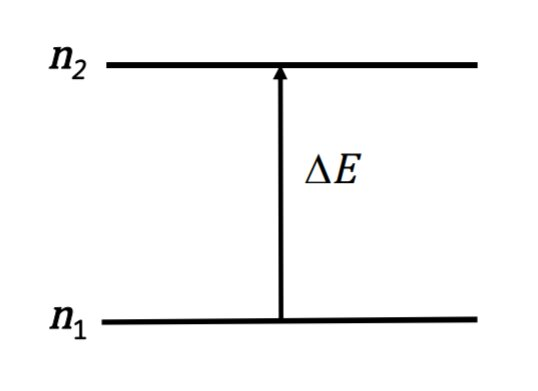
\includegraphics[width=4cm]{delte.jpg}
    \end{figure}

    The change in energy of an electron when changing level is 
    $$\Delta E = Z^2R_X\left(\frac{1}{n{_1} ^2}-\frac{1}{n{_2}^2}\right)$$
    When changing energy we can change $n$ however we like, however $l$ is restriced to only $\pm l$.
    So we can go from 1s to 3p, however not to 2s or 3d etc.

    How do we calculate the ionisation energy (IE) of a Hydrogen atom (Z = 1)? An atom is ionised when n $\rightarrow \infty$, so
    $$IE = \Delta E = 1^2R_H\left(\frac{1}{1^2}-\frac{1}{\infty^2}\right) = R_H$$

    \subsection{Angular Momenta}

    For a spectra of atoms/ions with more than one electron each electron will have its own set of 
    $n, l, m_l, s \text{ and } m_s$. The angular momenta ($l$) of different electrons can couple together in different ways
    which will have different energies. Since they determine the energy levels they determine spectroscopy i.e. lines we see on a spectrum.
    Considering different spins and angular momenta is called Russel-Saunders coupling.

    \subsubsection{Coupling Spin}
    Consider two electrons, 1 and 2, each has $s_1 = s_2 = \frac{1}{2}$ and $m_s = +\frac{1}{2}$ or $-\frac{1}{2}$
    If $S$ is the overall spin of the two electron system then the allowed values from from the Clebsch-Gordan series:
    \begin{center}
        \begin{math}
            S = s_1 + s_2 ,\ (s_1 + s_2)-1 \ ... \ |s_1 - s_2|
        \end{math}
    \end{center}
    So the allowed  values of $S$ are $\frac{1}{2} + \frac{1}{2} = 1$ and $\frac{1}{2} - \frac{1}{2} = 0$

    \subsubsection{Coupling Orbital Angular Momenta}
    Again, consider two electrons, they will have orbital angular momenta of $l_1$ and $l_2$. The value
    of these could be any real positive integer, $0, 1, 2...$ If $L$ is the total orbital angular momenta 
    of the combined system then the allowed values again come from the Clebsch-Gordan series:
    $$L = l_1 + l_2,\ (l_1 + l_2) - 1,\ (l_1 + l_2) - 2,/ ...\ |l_1 - l_2|$$
    So if $l_1 = 2$ and $l_2 = 3$ then we have a highest value of $2+3=5$ and a lowest value of $|2-3| = 1$.
    So L has a range of values of $L = 5, 4, 3, 2, 1$

    \subsubsection{Coupling Spin and Orbital Angular Momenta}
    We have $S$ and $L$ for a two-electron atom, we can combine these to get the allowed values of the 
    spin-orbit angular momentum, $J$. Unsurprisingly we use a Clebsch-Gordan series:
    $$J = L + S,\ L+S-1,\ ...\ |L-S|$$
    So if both $L$ and $S$ are 1, then the allowed values of $J$ are 2, 1 and 0

    \subsubsection{Many electron atom}
    For any electron in a many-electron atom it will have its own values of $l,\ m_l,\ s,\ m_s,\ j$.
    However the system as a whole (the entire atom) will have its own values of $L,\ M_L,\ S,\ M_S,\ J$.
    \begin{align*}
        M_L &= L,\ L-1,\ ...\ -L\\
        M_S &= S,\ S_1,\ ...\ -S \\
        M_L &= \sum m_l \\
        M_S &= \sum m_s 
    \end{align*}

    \subsection{Atomic term symbols and transitions}
    {\huge $$^{2S+1}L_J \quad \text{e.g.} \quad ^{2}P_{\frac{3}{2}}$$}

    \begin{itemize}
        \item $2S+1$ is the "spin multiplicity, S is the total spin quantum number for the atom
        \item $L$ is the total orbital angular momentum quantum number for the atom
    \end{itemize}
    In the same vein of s, p, d and f orbitals the same applies to $L$
    \begin{align*}
        S: L &= 0 \\
        P: L &= 1 \\
        D: L &= 2 \\
        F: L &= 3
    \end{align*}
    \begin{itemize}
        \item $J$ is the total angular momentum quantum number for the atom, i.e. how L and S are coupled
    \end{itemize}
    % \begin{center}
    % \begin{modiagram}[style=square, AO-width=20pt]
    %     \AO{s}[label={$m_l = 1$}]{0;up}
    %     \AO(40pt){s}[label={$m_l = 0$}]{0;up}
    %     \AO(80pt){s}[label={$m_l = -1$}]{0;up}
    %   \end{modiagram}
    % \end{center}

    A p-orbital has $l=1$, thus $m_l = +1, 0, -1$, instead of using $p_x, p_y, p_z$ we will use the $m_l$ numbers instead.

    \begin{center}
        \begin{modiagram}[style=square, AO-width=20pt]
            \AO{p} [label[x]={$m_l=+1$}, label[y]={$m_l=0$}, label[z]={$m_l=-1$}] {0;up,up,up}
        \end{modiagram}
    \end{center}
    
    Electron spin is represented with up\ ($m_s = +\frac{1}{2}$) and down\ ($m_s = -\frac{1}{2}$) arrows
    \begin{modiagram}[style=square]
        \AO{s}{0;pair}
    \end{modiagram}

    \subsubsection{Closed-shell atoms}
    A closed (sub)shell atom is any atom for which all of the electrons are paired. 

    \begin{center}
        \begin{modiagram}[style=square, AO-width=15pt]
            \AO{s}[label={$m_l = 0$}]{0;pair}
        \end{modiagram}
        \begin{align*}
            M_s = \sum m_s = S, S-1, ... -S
        \end{align*}
    \end{center}
    
    Well we know for He that we have two electrons, where $m_s = \pm \frac{1}{2}$ so $M_S$ = 0. This is the 
    only value we could have for He so $S = 0$ as well. This is true for every closed shell atom (like the Noble gasses).
    \begin{center}
        \begin{align*}
            M_L = \sum m_l = L, L-1, ... -L
        \end{align*}
    \end{center}
    For an s orbital $l = 0$ and so $m_l = 0$ as well, thus $M_L = 0$, this also means that $L=0$ for helium, 
    and as such $J=0$ too, we know this from the equations above. This is true for all closed shell atoms.
    So our term symbol for He is thus $^1S_0$, this is read as ``singlet S 0'', this is the same for all closed shell atoms,
    e.g. Ne, Li$^+$, Mg$^{2+}$, we call these singlet states.

    \subsubsection{Alkali Metal Atoms}
    We know they have a single unpaied electron in an s orbital     
    \begin{modiagram}[style=square]
        \AO{s}{0;up}
    \end{modiagram}

    So for Potassium, which has an electronic config of $\ce{[Ar] 4s^1}$, up until the 4s$^1$ shell it is a
    closed shell atom, and so overall it will have values $S = 0$ and $L = 0$. So we can consider it as a
    single unpaired electron, $m_s=\frac{1}{2}$ and so $s=\frac{1}{2}$ thus $S = \frac{1}{2}$. 
    The electron is in an s orbital, so $l = 0,\ m_l = 0$ hence $L = 0$.
    $$J = L+S,\ L+S-1\ ...\ |L-S| = 0 + \frac{1}{2}, |0-\frac{1}{2}| = \frac{1}{2}$$
    $$^2S_{\frac{1}{2}}$$
    This term symbol is the same for all Alkali metal atoms, since the only difference between them is the size
    of the closed shell, which always gives 0. The same applies to other elements with a closed shell before a ns$^{1}$
    electronic config, like Copper. $\ce{[Ar] 3d^10 4s^1}$
    \newline

    What happens if we excite an alkali metal atom so that the outermost s orbital electron is moved up into a p orbital?
    For potassium that would give a configuration of $\ce{[Ar] 4p^1}$ 
    \begin{center}
        \begin{modiagram}[style=square, AO-width=20pt]
            \AO{p} [label[x]={$m_l=+1$}, label[y]={$m_l=0$}, label[z]={$m_l=-1$}] {0;up,0,0}
        \end{modiagram}
    \end{center}
    We can forget about [Ar] since they only give 0, and so $s =\frac{1}{2},\ m_s=\frac{1}{2},\ S=\frac{1}{2}$.
    But now the electron is in a p orbital so $l=1,\ L=1$. 
    $$J = L+S,\ L+S-1\ ...\ |L-S| = \frac{3}{2},\ \frac{1}{2}$$
    So now we have two term symbols, these are two different electronic states that will have different energies.
    This will give us two different states in spectroscopy. Since $2S+1 = 2$ we call these states ``doublet'' states.
    {\large $$^2P_\frac{3}{2} \quad \text{and} \quad ^2P_\frac{1}{2}$$}

    \subsubsection{What do we see in the spectrum?}
    We have selection rules, $\Delta J = 0, \pm 1$, we can leave J unchanged (but not going from 0 to 0), but we have to change our orbital, i.e. l has to change, 
    this is due to photons having an angular momentum. $\Delta S = 0$, since photons have no spin.
    \newline

    So when we promote, say, a Sodium atom, from 3s to 3p the term symbol goes from $^2S_\frac{1}{2}$ to either
    $^2P_\frac{3}{2}$ or $^2P_\frac{1}{2}$, these two final states are slightly different in energy. 
    We can confirm our that changes are valid, $S = \frac{1}{2}$ does not change on the transition to/from
    the s/p orbital. However $J$ does change, but only for $\Delta J = 0, 1$, so it is valid. 

    The intensity of the transition is determined by the relative degeneracy of the upper levels, which is 
    $2J+1$. So we have a ratio of 2:1 for our transitions of Sodium. The 3 infront of the term symbols is 
    the energy level i.e. 3 
    \begin{align*}
        3^2P_\frac{3}{2} \rightarrow 3^2P_\frac{1}{2} \quad 2\cdot \frac{3}{2} &= 4\\
        3^2P_\frac{1}{2} \rightarrow 3^2P_\frac{1}{2} \quad 2\cdot \frac{1}{2} &= 2
    \end{align*}

    What happens if we transition Sodium to a 4d$^1$ orbital? This will give an electronic config of $\ce{[Ne] 4d^1}$
    \begin{align*}
        s &= \frac{1}{2},\ S=\frac{1}{2}\\
        l &= 2,\ L = 2\\
        J &= L + S,\ ... \ |L-S| = \frac{5}{2},\ \frac{3}{2}
    \end{align*}

    We cannot have a transition from $^2D_\frac{5}{2}$ to $^2P_\frac{1}{2}$ as $\Delta J = 2$ which breaks our selection rules.
    $^2D_\frac{5}{2}$ and $^2D_\frac{3}{2}$ are very close in energy and so if the resolution of our equipment 
    isn't low enough we may see only 2 peaks for the transitions from d to p, this is always something to consider.

    \begin{figure}[h]
        \centering
        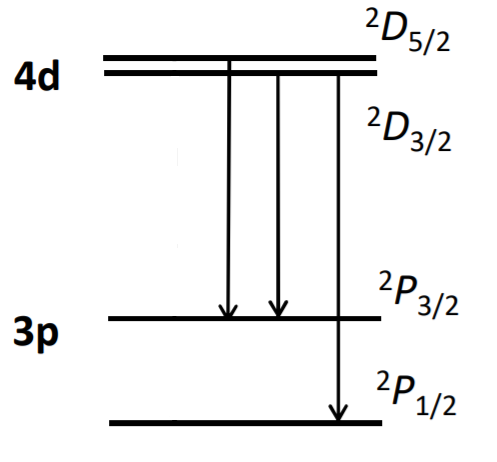
\includegraphics[width=6cm]{4d.png}
    \end{figure}

    \subsection{More Atomic Term Symbols}

    Consider a Carbon atom in its ground state $\ce{[Be] 2p^2}$, so we have $s_1 = s_2 = \frac{1}{2}$ thus $S = 0, 1$
    \begin{center}
        \begin{align*}
            s_1 = s_2 = \frac{1}{2} \quad \text{thus}  \quad S &= 0, 1\\
            l_1 = l_2 = 1 \quad \text{thus}  \quad l &= 0, 1, 2\\
            ^1S,\ ^3S,\ ^1P,\ ^3P,\ ^1D,\ &^3D\ \text{Different ``states''}
        \end{align*}
    \end{center}
    Lets look closer at the $^3D$ term, $L=2$ and so it must have an $M_L = 2$ component, so we must have an $m_l = 1$ 
    for each electron as $\sum m_l = M_L$, and we have two electrons. For the triplet D state ($^3D$) it must have 
    $S = 1$ as $3 = 2S + 1$, so it must have an $M_S = 1$ component which means that $m_s = \frac{1}{2}$ for each electron.

    \begin{center}
        \begin{modiagram}[AO-width=20pt]
            \AO{p} [label[x]={$m_l=+1$}, label[y]={$m_l=0$}, label[z]={$m_l=-1$}] {0;up,0,0}
            \AO(5pt){s}{0; up}
        \end{modiagram}
    \end{center}

    This would mean that there would be two up ($m_s = \frac{1}{2}$) spin electrons with the same $m_l$, 
    they have the same quantum numbers,this violates the pauli exclusion principle.

    \subsubsection{Hund's Rules}
    Within Russell-Saunders coupling, for a given configuration, in its \textbf{ground state}:
    \begin{enumerate}
        \item The term with the largest S is lowest in energy
        \item For a given S the term with the largest L is lowest in energy
        \item For a term with several levels:
        \begin{itemize}
            \item if the sub-shell is less than half full  then the lowest $J$ level is the lowest in energy
            \item if the sub-shell is more than \textbf{or} half full then the highest $J$ level is lowest in energy
        \end{itemize}
    \end{enumerate}

    To find the ground state of a Carbon atom we work through these rules. 
    \begin{enumerate}
        \item Largest $S$ (and so largest $M_S$), so parallel spins ($m_s$ are the same)
        \begin{itemize}
            \item $S = \frac{1}{2} + \frac{1}{2},\ \frac{1}{2}-\frac{1}{2},\ =\ 1,\ 0$
            \item $M_S = \frac{1}{2} + \frac{1}{2} = 1$
        \end{itemize}
        \item For a given $S$, largest $L$ (and so largest $M_L$), so the two highest $m_l$ are needed
        \begin{itemize}
            \item $m_l = 1,\ 0$
            \item $M_L = 1 + 0 = 1 = L$
        \end{itemize}
        \item $J = L+S,\ L+S-1,\ ...\ |L-S| = 2, 1, 0$
        \begin{itemize}
            \item Since our orbital is less than half filled then J must take the lowest value, so $J=0$
        \end{itemize}
    \end{enumerate}

    \begin{center}
        \begin{modiagram}[style=square, AO-width=20pt]
            \AO{p} [label[x]={$m_l=+1$}, label[y]={$m_l=0$}, label[z]={$m_l=-1$}] {0;up,up,0}
        \end{modiagram}
    \end{center}

    Putting this all together gets the ground state of Carbon to be $^3P_0$
    \newline

    This is similar to Carbon. We have two extra electrons, obeying Hund's rules we add it to $m_l = -1$
    with the same spin as the other two, and then with the one left over it has to have the opposite spin but
    go with the highest $m_l$. Our orbital is now more than half full and so we must go with the highest $J$ value.
    $^3P_2$
    \begin{center}
        \begin{modiagram}[style=square, AO-width=20pt]
            \AO{p} [label[x]={$m_l=+1$}, label[y]={$m_l=0$}, label[z]={$m_l=-1$}] {0;pair,up,up}
        \end{modiagram}
    \end{center}

    Now let us consider a Nitrogen atom, $\ce{[Be] 2p^3}$. Obeying the first rule we know they should all have 
    parallel spins so $m_s = +\frac{1}{2}$ for each electron. Obviously they all need different $m_l$ values.
    $M_S = 3\frac{1}{2} = \frac{3}{2}$ and $M_L = 1 + 0 - 1 = 0$. So we take the highest $S$ value, $\frac{3}{2}$
    and the highest $L$ value, $0$, which means that $J = \frac{3}{2} + 0$, we take the highet $J$ value since
    our shell is only half full. $^4S_\frac{3}{2}$
    \begin{center}
        \begin{modiagram}[style=square, AO-width=20pt]
            \AO{p} [label[x]={$m_l=+1$}, label[y]={$m_l=0$}, label[z]={$m_l=-1$}] {0;up,up,up}
        \end{modiagram}
    \end{center}
    \newpage

    Consider a Fluorine atom now, this is symmetrically similar to Boron.
    \begin{center}
        \begin{modiagram}[style=square, AO-width=20pt]
            \AO{p} [label[x]={$m_l=+1$}, label[y]={$m_l=0$}, label[z]={$m_l=-1$}] {1.5;pair,pair,up}
            \AO{p} [label[x]={$m_l=+1$}, label[y]={$m_l=0$}, label[z]={$m_l=-1$}] {0;up,0,0}
        \end{modiagram}
    \end{center}
    For Fluorine we have 
    \begin{itemize}
        \item $M_S = 3\frac{1}{2} - 2\frac{1}{2} = \frac{1}{2} = S$
        \item $M_L = 1 + 0 - 1 + 1 + 0 = 1 = L$
        \item $J = \frac{3}{2},\ \frac{1}{2}$
    \end{itemize}
    Since this has one unpaired electron we will get the same term ($^2P$) as a single unpaired electron.
    And now we just need to consider if the subshell is half full or half empty for our J value.
    \begin{itemize}
        \item $M_S = \frac{1}{2} = S$
        \item $M_L = 1 = L$
        \item $J = \frac{3}{2},\ \frac{1}{2}$
    \end{itemize} 
    For Boron $^2P_\frac{1}{2}$ and for Fluorine $^2P_\frac{3}{2}$, this is a very useful symmetry, that would
    also apply for two unpaired electrons.

    \subsubsection{Examples}
    Term symbols for Arsenic, Phosphorus and Selenium$^+$. Notice how they all have the same electronic configuration
    after the closed shells, p$^3$. This means they're isoelectric and so will have the same term symbol.
    \begin{itemize}
        \item $M_S = 3\frac{1}{2} = \frac{3}{2} = S$
        \item $M_L = 1 + 0 - 1 = 0 = L$
        \item $J = \frac{3}{2}$
        \item $^4P\frac{3}{2}$
    \end{itemize}

    Another example for Cl, Cl$^{-}$, Cl$^+$. They are no isoelectric and so will have different term symbols,
    not to worry. For Cl 3p$^{5}$, we can treat it like a single electron atom.
    \begin{itemize}
        \item $M_S = \frac{1}{2}$
        \item $M_L = 1$
        \item $J = \frac{3}{2},\ \frac{1}{2}$
        \item Since the subshell is more than half full we use the highest $J$ value
        \item $^2P_\frac{3}{2}$
    \end{itemize}
    Cl$^{-}$ has one more electron, thus making it a closed shell ion, so it will be $^1S_0$. 
    Cl$^{+}$ has a config of 3p$^4$, we can treat this as a two unpaired electron atom.
    \begin{itemize}
        \item $M_S = 1$
        \item $M_L = 1$
        \item $J = 2,\ 1,\ 0$
        \item Since the subshell is more than half full we use the highet $J$ value
        \item $^3P_2$
    \end{itemize}

    \section{Rotational Spectroscopy}\thedate{Week 3}

    For a diatomic molecule, the masses of the two nuclei are $m_1$ and $m_2$. We can instead model this as
    as single atom of mass $\mu$ rotating a distance $R$ away from its axis. $I = \mu R^2$, I is the moment of 
    inertia, it is the rotational equivalent to mass.

    \begin{figure}[h]
        \begin{center}
            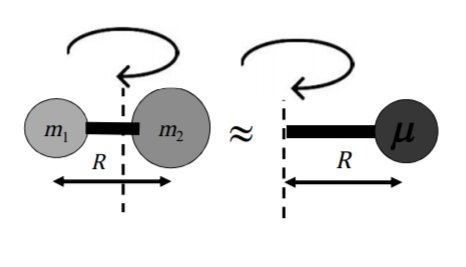
\includegraphics[width=5cm]{rotat.jpg}
        \end{center}
    \end{figure}

    If we solve the Schr{\"o}dinger equation for rotational motion and find the eigenvalues (energies).
    We get an expression, where $F(J)$, or $E_J$, is the rotational energy, $J$ is the rotational quantum number,
    where $J = 0, 1, 2, 3...$ and $B$ is the rotational constant given by $B = \frac{\hbar^2}{2I}$, it depends 
    on the molecule. 
    $$F(J) = E_J = BJ(J+1)$$
    For molecules with Hydrogen we get values in the $10-100$\cm range, but without Hydrogen they are single
    digited. There is obviously no energy when there is no rotation, $F(0) = 0$. With each increasing $J$ the
    energy levels space out more because of the $J^2$ term in $F(J)$

    \subsection{The Rotational Constant $B$}
    Although $B$ should be given in Joules, in microwave (rotational) spectroscopy we use Hertz. 
    \begin{align*}
        B (\text{J}) &= \frac{\hbar^2}{2I} = \frac{h^2}{8\pi^2I} \qquad \text{since } E = hf\\
        B (\text{Hz}) &= \frac{h}{8\pi^2I} \qquad \text{since } E = \frac{hc}{\lambda}\\
        B (\text{cm}^-1) &= \frac{h}{8\pi^2I\tilde{c}} \qquad \tilde{c} \text{ is c in cm s}^-1
    \end{align*}

    \subsection{Rotational Selection Rules}
    A molecule must have a permanent dipole moment for it to exhibit a pure rotational (microwave) spectrum.
    It cannot be linear e.g. \ce{CO2}, however it can be linear and asymmetric, e.g. \ce{N2O} which is \ce{N-N-O}
    Transitions can only change by 1, i.e. $\Delta J = \pm 1$ 
    \begin{align*}
        F(J) &= BJ(J+1)\\
        \Delta F(J) = \tilde{\nu}(J) &= F(J+1) - F(J)\\
        &= B(J+1)(J+2) - BJ(J+1)\\
        &= 2B(J+1)
    \end{align*}
    So the transitions that we see on a microwave spectrum will be equally spaced by $2B$. We do not see 
    any transitions from rotations about the axis that goes \emph{through} the molecule. Rotations from the other
    two axes are indistinguishable from each other, they are degenerate. \\

    $B \propto \frac{1}{I} = \frac{1}{\mu R^2}$ Thus we can get an accurate value for bond length through 
    microwave spectroscopy. $B$ is isotope dependent, so so two isotopes will have different spacings.
    In the absence of any external fields, for each $J$ level there are $2J+1$ levels with the same energy (degenerate)
    for each $J$ level, this comes from the $M_J$ projection quantum number, we will assume there is no external
    field.

    \subsection{Populations of the rotational levels}
    From the Boltzmann distribution $$n_J \propto g_J exp\left(-\frac{F(J)}{k_BT}\right) = (2J+1)exp\left(-\frac{BJ(J+1)}{k_BT}\right)$$
    We saw earlier that the degeneracy for each $J$ is $g_J = (2J +1)$ and $F(J) = BJ(J+1)$

    The most populated level occurs at the turning point of the function, so $\dv*{n_J}{J}=0$
    $$\dv{n_J}{J} = \left(2 -(2J+1)^2\frac{B}{k_BT}\right)exp\left(-\frac{BJ(J+1)}{k_BT}\right) = 0$$
    Since an exponential cannot be zero except for at negative infinity the term that must go to zero is its
    coefficient.
    \begin{align*}
        2 &- (2J_{\text{max}} + 1)^2\frac{B}{k_BT} = 0\\
        J_\text{max} &= \sqrt{\frac{k_BT}{2B}} - \frac{1}{2}\\
    \end{align*}

    \subsection{Centrifugal distortion}
    Are molecules rigid? Unfortunately, no. As the molecule is rotated the atoms move further apart, so $I$ will
    change with $J$. However this is small enough that we can account for it in a clever way.
    $$ F(J) = BJ(J+1) - D(J(J+1))^2$$
    $D$ is the centrifugal distortion constant, in \cm $^{-1}$. D is very small, ($10^{-5} - 10^{-3}$).
    As $J$ increases the \emph{centrifugal distortion} caused by the non-rigidness will get bigger and bigger and bring 
    down $F(J)$ more, causing it to deviate the higher $J$ gets.\\

    The tranistions (spacing between the levels, wavenumber) when accounting for centrifugal distortion
    \begin{align*}
        \Delta F(J) = \tilde{\nu}(J) &= F(J+1) - F(J) \\
        &= 2B(J+1) - 4D(J+1)^3\\
        \frac{\tilde{\nu}(J)}{J+1} &= 2B-4D(J+1)^2
    \end{align*}

    From this we can form a plot, where $y = \frac{\tilde{\nu}(J)}{J+1}, x = (J+1)^2$, the y-intercept is $2B$
    and the \emph{gradient} is $-4D$

    \newpage

    \subsection{Vibrational Frequency}
    Since the molecule stretches slightly when rotating, we can deduce something about the strength of the bond.
    This is called the vibrational frequency, $\omega_e$, it can be shown (but we won't) that
    $$\omega_e^2 = \frac{4B^3}{D}$$ 

    \subsubsection{Example}
    The pure rotational spectrum for HI has been measured and has lowest observed line poistions as follows.

    \begin{tabular}{l}
        $\Delta F(J) / \text{cm}^{-1}$ \\
        \hline
        12.8519\\
        25.6877\\
        38.5358\\
        51.3580\\
        64.1602\\
        76.9376\\
        89.6852\\
    \end{tabular}

    So we need to plot $\frac{\Delta F(J)}{J+1}$ against $(J+1)^2$, where $2B$ will be the intercept and $-4D$ the slope.

    \begin{tabular}{l l}
        $\frac{\Delta F(J)}{J+1}$ & $(J+1)^2$\\
        \hline
        12.8519 & 1\\
        12.8494 & 4\\
        12.8452 & 9\\
        12.8494 & 16\\
        12.8320 & 25\\
        12.8229 & 36\\
        12.8121 & 49
    \end{tabular}
    \begin{figure}[h]
        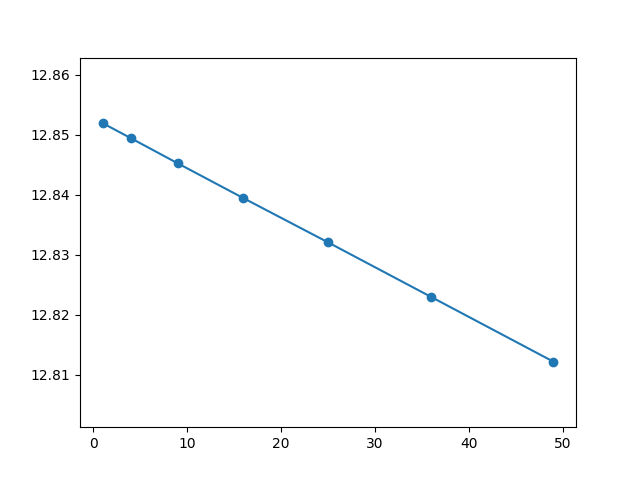
\includegraphics[width=8cm]{Figure_1.png}
    \end{figure}

    From this plot we can derive our gradient and intercept and get $B = 6.4265 \text{cm}^{-1}$ and \\$D=2.069 \times 10^{-4} \text{cm}^{-1}$
    so $\omega_e = 2265 \text{cm} ^{-1}$

    \subsubsection{Practice}
    \begin{itemize}
        \item \ce{H2} has no rotational spectra because it does not have a dipole moment.
        \item \ce{HBR} has a rotational spectra because it has a dipole moment.
        \item \ce{CO2} has no rotational spectra because it is linear.
        \item \ce{H2O} has a rotational spectra because it is not linear.
        \item \ce{N2O} has a rotational spectra because despite being linear, it is asymmetric, \ce{N-N-O}
        \item Cis-dichloromethane has a spectra because because the chlorines are on one end, so the mass is unbalanced.
        \item Trans-dichloromethane has no spectra because the chlorines are on either end, so the mass is balanced. 
        \item A symmetric molecule like \ce{BF3} will not have a spectra because the mass is balanced, all the fluorides cancel out.
    \end{itemize}
    
    \section{Harmonic and anharmonic vibrations}\thedate{Week 4}

    Some confusing preliminary knowledge:
    \begin{itemize}
        \item $\omega_e$ \cm is the vibrational wavenumber (the vibratioanl frequency in \cm), we saw in the previous section
        \item $\omega$ is the angular frequency
        \item $\nu$ (NOT v) or $\nu_\text{vib}$ is the vibrational frequency
        \item $\omega = 2\pi \nu$
        \item $\hbar \omega = h \nu$
        \item $\omega_e$ has units \cm whilst $h\nu$ has units J, we can sub one in for the other, to change 
        the units, so if the energy is given in \cm we use $\omega_e$
        \item To get $\omega_e$ in J we do $h\tilde{c}\omega_e = h\nu$, since they are both in Joules, so $\omega_e = \frac{\nu}{\tilde{c}}$
    \end{itemize}


    We can assume that molecules obey Hooke's Law, $F= - k_Fx$, $V = -\int F \text{d}x$, so that \emph{classical} harmonic frequency of 
    oscillation is $\nu_\text{vib} = \frac{1}{2\pi}\sqrt{\frac{k_F}{\mu}}$, where $\nu_\text{vib}$ is the 
    vibrational frequency. 
    If we solve the Schr{\"o}dinger equation for harmonic motion, we can find the vibrational wavenumber, 
    $\omega_e \mcm$ and vibrational frequency $h\nu_\text{vib}$ J
    $$\omega_e = \frac{\nu_\text{vib}}{\tilde{c}} = \frac{1}{2\pi\tilde{c}}\sqrt{\frac{k_F}{\mu}} \mcm$$
    So the energy levels that arise (similar to $F(J)$), where $v$ (NOT $\nu$) is the vibrational quantum number, $v = 0, 1, 2...$
    $$G(v) = \left(v + \frac{1}{2}\right)\omega_e$$
    Remember how for $F(J)$ when $J = 0$ then $F(0) = 0$, however for vibrational motion this is not the case.
    $G(0) = \frac{1}{2}\omega_e \neq 0$. So the energy levels start at $\frac{1}{2}\omega_e$ and are spaced evenly
    from there e.g. $G(1) = \frac{3}{2}\omega_e$, the gap between each is $\hbar\omega$ or $h\nu$ is measured in Joules.

    \begin{figure}[h]
        \centering
        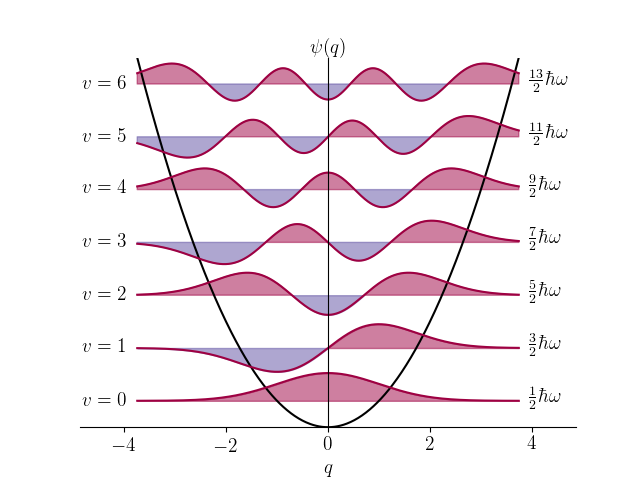
\includegraphics[width=6.5cm]{vib.png}
        \caption{Haromic oscillator wavefunctions}
    \end{figure}

    \subsection{Anharmonicity}
    
    Molecular bonds are not harmonic oscillators, we can not increase the frequency indefinitely, as the bond stretches
    and gets longer it will eventually reach dissociation energy and fall apart. So for \ce{HCl} it will split into
    H and Cl \emph{atoms}

    \begin{figure}[h]
        \centering
        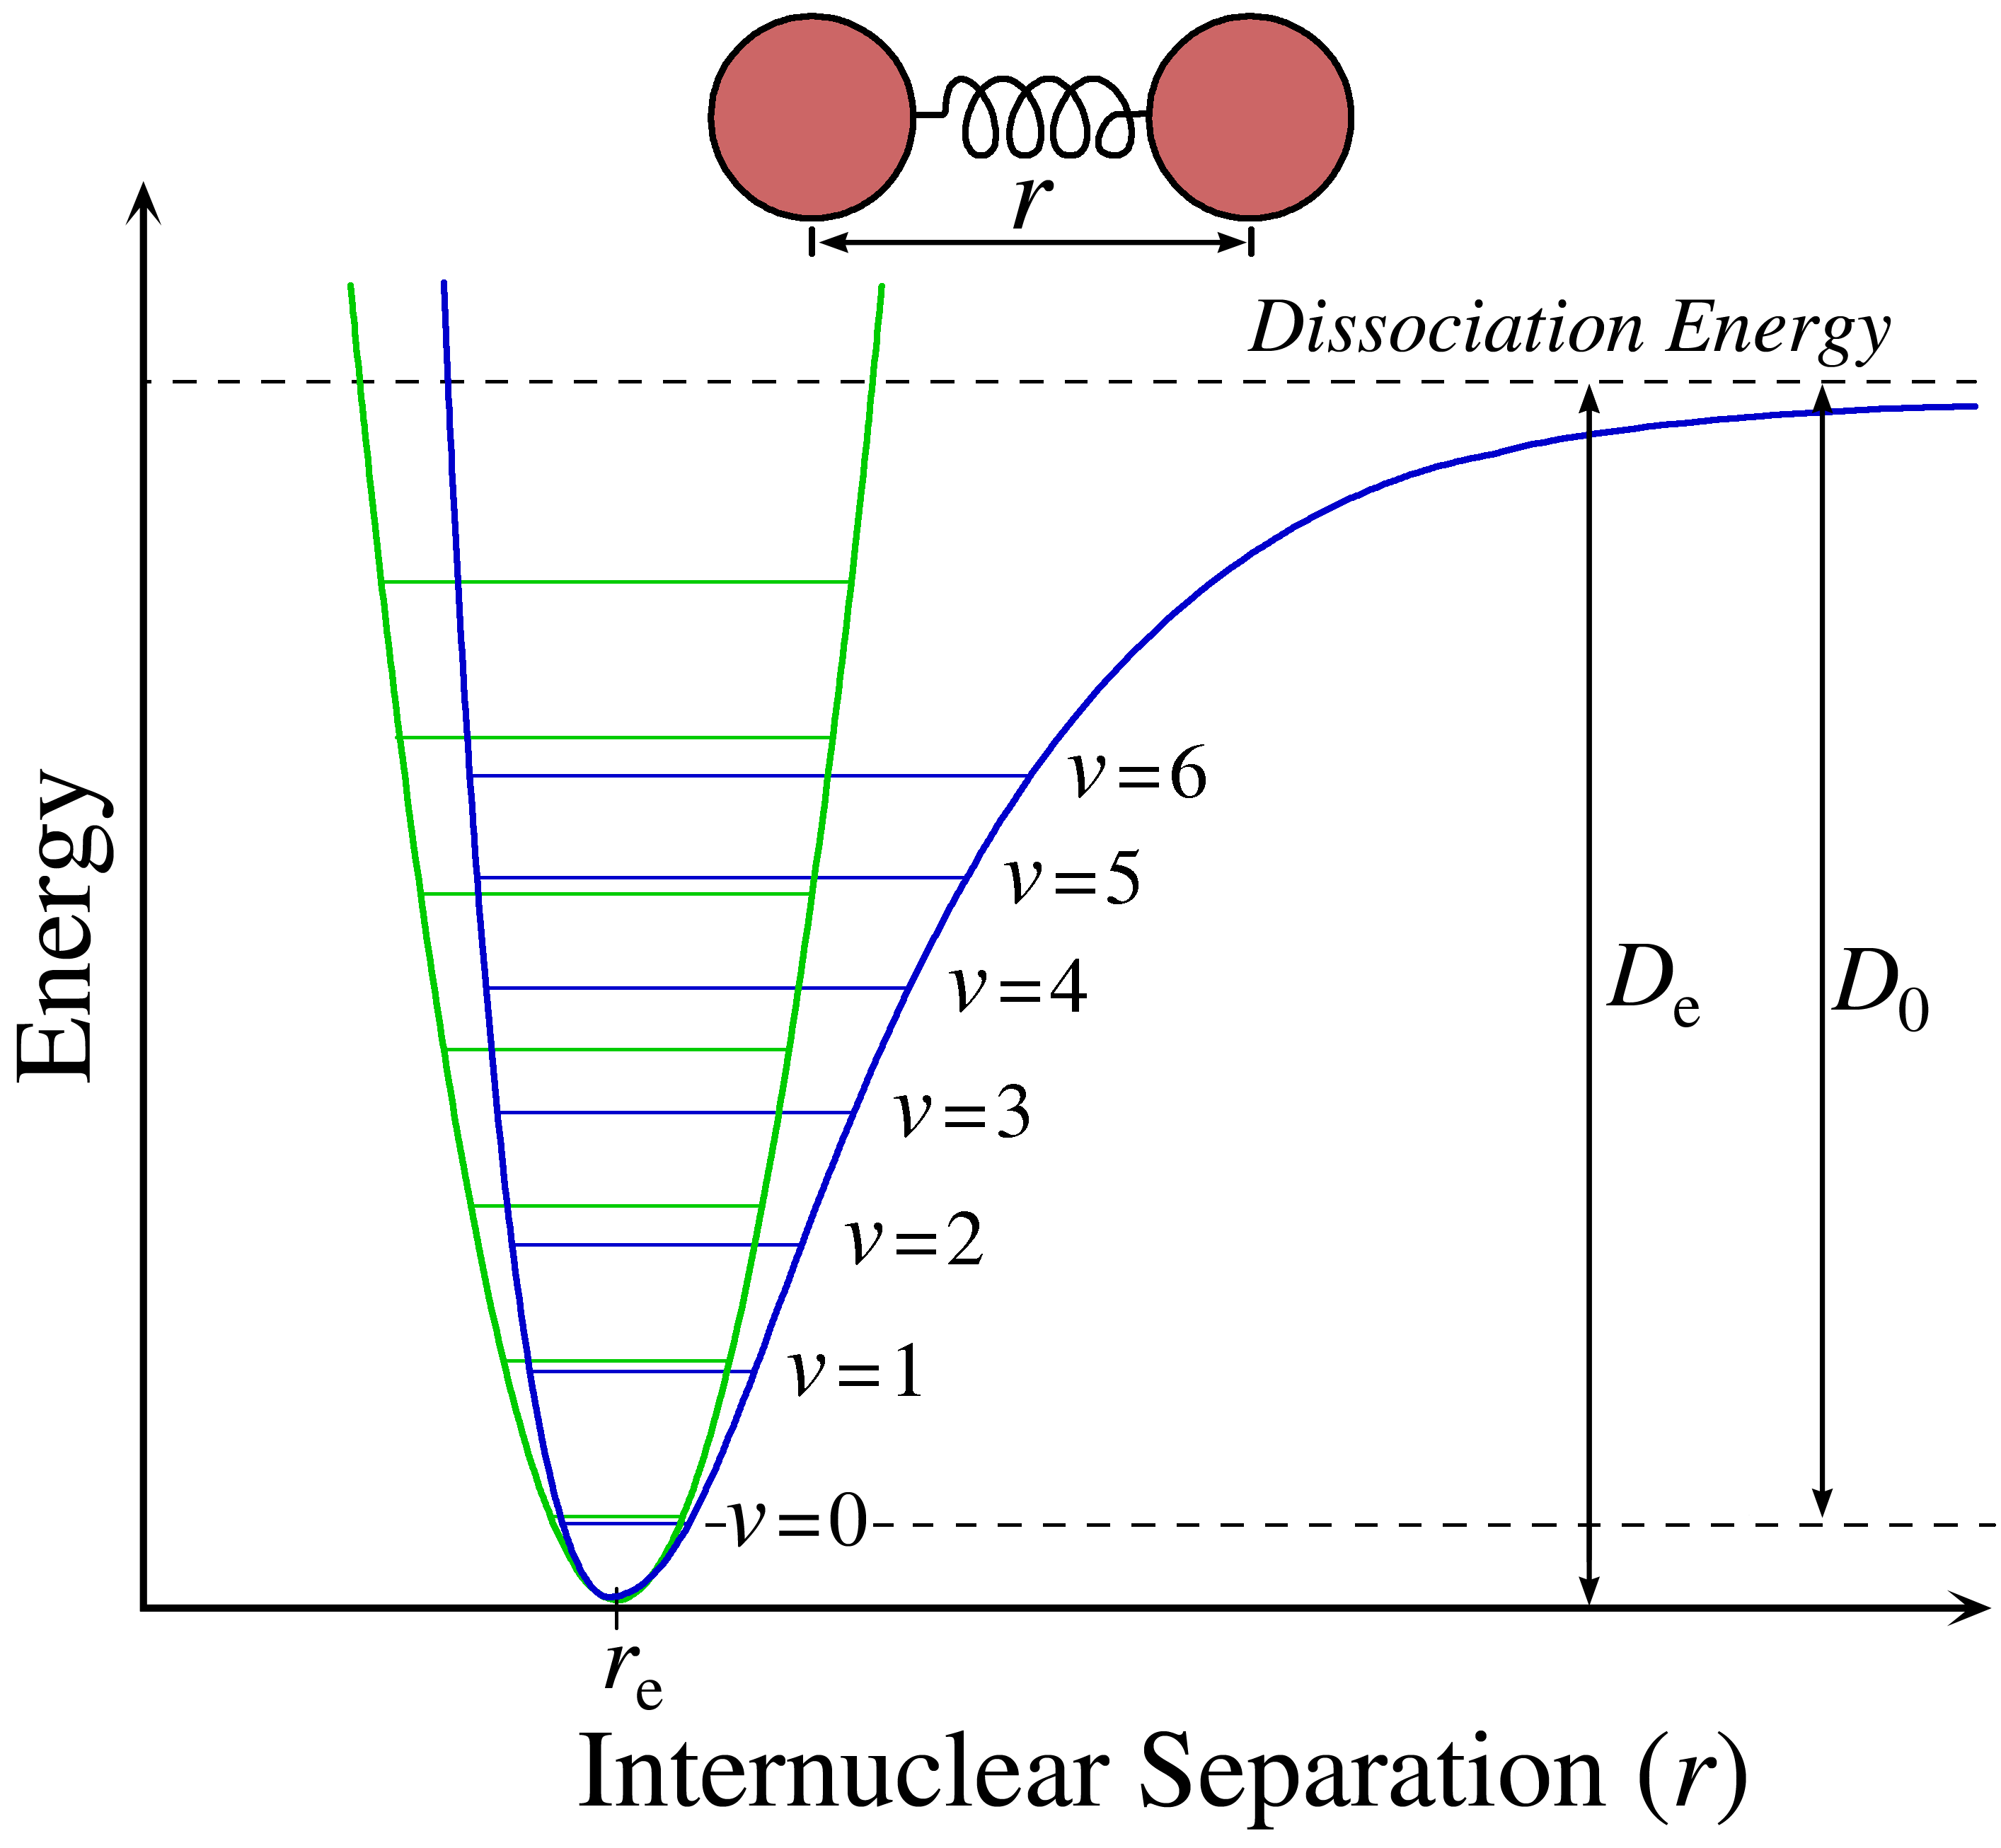
\includegraphics[width=6.5cm]{dis.png}
    \end{figure}

    We describe the \emph{anharmonic} oscillations using the morse potential (the blue on the above diagram).
    $$V(R) = D_e\left(1 - exp(-\beta(R-R_e))\right)^2$$
    $D_e$ is the dissociation energy, however since the molecule always vibrates we can't measure this (remember
    that $G(0) \neq 0$), so instead we have to measure $D_0 = D_e - G(0)$.

    \subsubsection{Anharmonic oscillator transitions}
    $$G(v) \text{ or } E(v) \text{ or } \tilde{\nu} = (v + \frac{1}{2})\omega_e - (v+\frac{1}{2})^2\omega_e x_e$$
    
    $x_e$ is the dimensionless anharmoninicity constant, however we normally talk about this constant in the form 
    of $\omega_e x_e$. We need a dipole moment during the vibration, so only hateronuclear diatomics will work. 
    \begin{itemize}
        \item Harmonic oscillator $\Delta v = \pm 1$
        \item Anharmonic oscialltor  $\Delta v = \pm 1, 2, 3...`'$
    \end{itemize}
    The transitions can be calculated by $\tilde{\nu}(2) - \tilde{\nu}(0)$.
    \begin{itemize}
        \item fundamental $(0 \rightarrow 1)\ \tilde{\nu}  = \omega_e - 2\omega_e x_e \mcm$
        \item 1st overtone $(0 \rightarrow 2)\ \tilde{\nu} = 2\omega_e - 6\omega_e x_e \mcm$
    \end{itemize}

    \subsection{Vibration-rotation spectroscopy}

    As we saw in a graph at the beginning, each vibrational transition has many rotational transitions associated
    with it, however, they occur independently, and so we can add just add them together. $E_\text{tot} = E_\text{vib} + E_\text{rot}$
    We denote this energy by $S(v, J) = G(v) + F(J)$ 

    $$S(v, J) = \left(v + \frac{1}{2}\right)\omega_e - \left(v + \frac{1}{2}\right)^2\omega_e x_e + B_vJ(J+1)$$

    \begin{itemize}
        \item All $\Delta J = +1$ transitions give to rise an R-branch absorption, they have a higher wavenumber than $\tilde{\nu}_0$
        \item All $\Delta J = -1$ transitions give rise to a P-branch absorption, they have a lower wavenumber than $\tilde{\nu}_0$
    \end{itemize}
    $\tilde{\nu}_0 = \omega_e - 2\omega_e x_e$ i.e. $\tilde{\nu}_0 = S(1, 0) - S(0, 0)$
    
    \begin{figure}[h]
        \centering
        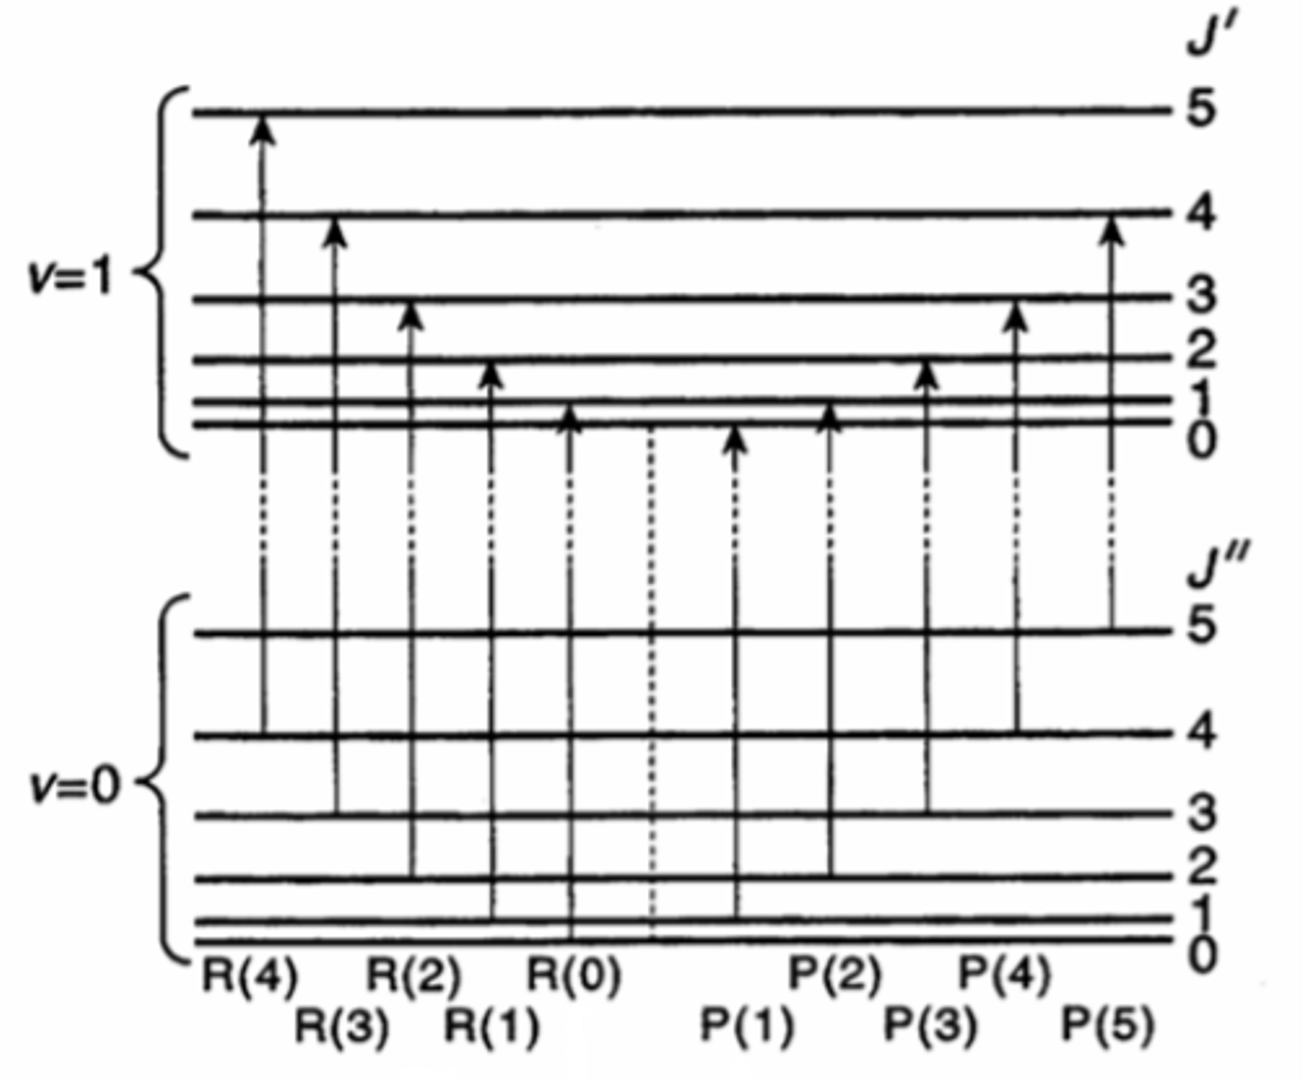
\includegraphics[width=6.5cm]{vj.png}
    \end{figure}

    We can see the different types of transitions (R on the left, P on the right). The energy associated with any
    vibrational transition ($v$) is the same no matter the rotational transition ($J$). For any transition we call 
    the lower rotational energy $J''$ and the higher level $J'$, so for some generic transition.
    $$\Delta \tilde{\nu} = S(v', J') - S(v)'', J'')$$
    Take for example a vibrational transition in the fundamental vibrational band ($0 \rightarrow 1$), for any 
    $J$ values the vibrational energy is always $\omega_e - 2\omega_e x_e$, so we only have to worry about the rotational
    transition. Calculating for some generic $\tilde{\nu}$ in the fundamental vibrational band i.e. $J$ goes 
    from $J''$ to $J'$. For $\tilde{\nu}_R$ tranistions we can say that $J' = J'' + 1$ (look at the above graph).

    \begin{align*}
        \tilde{\nu}_R (J'') &= S(1, J') - S(0, J'') = G(1) - G(0) + F(J') - F(J'') \\
        &= \omega_e - 2\omega_e x_e + F(J') - F(J'')\\
        \Delta F = F(J') - F(J'') &= B_1J'(J'+1) - B_0J''(J'' + 1)\\
        J' &= J'' + 1\\
        \Delta F &= B_1(J''+1)(J''+2) - B_0J''(J''+1)\\
        \tilde{\nu}_R &= \omega_e - 2\omega_e x_e + B_1(J''+1)(J''+2) - B_0J''(J''+1)
    \end{align*}

    For $\tilde{\nu}_P$ transitions in the fundamental vibrational band, $J'' = J'+1$, so the maths is slightly different,
    but only for the $\Delta F$ part.

    \begin{align*}
        \Delta F = F(J') - F(J'') &= B_1J'(J'+1) - B_0J''(J'' + 1)\\
        J'' &= J' + 1\\
        \Delta F &= B_1(J''+1)(J''+2) - B_0J''(J''+1)\\
        \tilde{\nu}_P &= \omega_e - 2\omega_e x_e + B_1(J''-1)(J'') - B_0J''(J''+1)
    \end{align*}

    If we assume that $B_1 = B_0 = B$ then we can say that the spacing between each branch is $2B$ and the central
    gap is $4B$
    \begin{figure}[h]
        \centering
        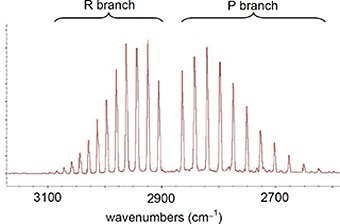
\includegraphics[width=5cm]{rbr.jpg}
    \end{figure}

    \newpage
    \subsection{Vibrational depedence of rotational constants}
    
    But is $B_1 = B_0$? For a harmonic oscialltor, which has symmetric energies, yes, it is. However for an
    anharmonic oscialltor where the distance changes this is not the case, the wavefunction skews up the well.
    We say $B \propto \frac{1}{\mu R^2}$, but R is changing with the vibration, so we need to consider
    $<\frac{1}{R^2}>$ for B. $<R^2>$ increases with $v$, so $<\frac{1}{R^2}>$ decreases with $v$, so
    $$B_0 > B_1 > B_{(v>1)}$$
    The rotational constant gets small the higher $v$ we go.
    $$B_v = B_e - \alpha\left(v + \frac{1}{2}\right)$$
    $B_e$ is the rotational constant for the bottom of the well, it needs to be calculated and can't be found experimentally.
    $\alpha$ is the vibration-rotation interaction constant. 
    This means that if we know $B_v$ for any two energy levels then we derive $B_e$ and $\alpha$\\

    We use tranistions with common upper or lower levels to determine the rotational constants.
    \subsubsection{From the same level}
    With two different transitions starting from the same J value, $J''$, at where $v$ goes $0\rightarrow1$.
    Since both of them have the same $v$ transition, when they are subtracted they will equal 0 so this simplifies
    the maths a lot. Since our transition equations are in the form of the initial $J$ value we can say.
    
    $$\nu_R(J) - \nu_P(J) = 2B_1(2J+1)\\$$

    And from this we can obtain our $B_1$

    \subsubsection{To the same level}
    It is very similar, but now our transitions end on the same level, since $\nu_R$ goes up and $\nu_P$ goes down 
    in J value, they must start like this.

    $$\nu_R(J-1) - \nu_P(J+1) = 2B_0(2J+1)$$

    What we can do for both of these is then plot a graph, where the slope is $B$ and from there we can calculate $B_e$ and $\alpha$

    \subsection{Example}
    HI molecule has its vibration-rotation spectrum measured, only four lines are given (\cm).

    \begin{tabular}{l l}
        $\tilde{\nu}$ & Difference\\
        2204.019\\
        & 13.021\\
        2217.040\\
        & 25.030\\
        2242.070\\
        &12.009 \\
        2254.079\\
    \end{tabular}

    We can see from the differences that one is double the others, that means that 2242 will be the $\tilde{\nu}_0$ line.
    The numbers lower than $R(0)$ are $P$ branches. 

    \begin{tabular}{l l}
        $\tilde{\nu}$ & Branch\\
        2204.019 & P(2)\\
        2217.040 & P(1)\\
        2242.070 & R(0)\\
        2254.079 & R(1)\\
    \end{tabular}

    Remember from our equations, that $\nu(J)$ uses the starting level, so to find $B_1$ we need levels with the 
    same $J$ value.
    \begin{align*}
        \nu_R(J) - \nu_P(J) &= 2B_1(2J+1)\\
        R(1) - P(1) &= 2254.079 - 2217.040 = 37.039\\
        &= 2B_1(2J+1) = 6B_1\\
        B_1 &= 6.1732
    \end{align*}

    For $B_0$ we need equations which end on the same level, or start two levels apart, luckily we have those too

    \begin{align*}
        \nu_R(J) - \nu_P(J) &= 2B_0(2J+1)\\
        R(0)-P(2) &= 38.051\\
        B_0 &= 6.3418
    \end{align*}

    Now we can find $B_e$ and $\alpha$ from our equations from before

    \begin{align*}
        B_v &= B_e - \alpha\left(v+\frac{1}{2}\right)\\
        B_0 &= B_e - \frac{1}{2} \alpha\\
        B_1 &= B_e - \frac{3}{2} \alpha\\
        B_0 - B_1 &= \alpha = 0.1686 \mcm\\
        B_e &= B_0 + \frac{1}{2}\alpha = 6.4261 \mcm\\
    \end{align*}

    We can now calculate the equilibrium bond length, $R_e$, recall that 

    \begin{align*}
        B_e \mcm &= \frac{h}{8\pi^2\mu R_e^2\tilde{c}}\\
        R_e &= \sqrt{\frac{h}{8 \pi^2 \mu \tilde{c}B_e}} \ \text{cm}\\
        &= 1.62 \ \text{\AA}
    \end{align*}

\end{document}